\documentclass[letterpaper,10pt,twocolumn]{article}

\usepackage[margin=0.75in]{geometry}
\usepackage{times}
\usepackage{helvet}
\usepackage{courier}
\usepackage{microtype}
\usepackage{graphicx}
\usepackage{amsmath,amssymb}
\usepackage{booktabs}
\usepackage{multirow}
\usepackage{array}
\usepackage{xcolor}
\usepackage{tikz}
\usepackage{url}
\usepackage{natbib}
\usepackage{enumitem}
\usepackage{caption}
\usetikzlibrary{arrows.meta,positioning,fit,calc,shapes.geometric}

\setlength{\pdfpagewidth}{8.5in}
\setlength{\pdfpageheight}{11in}
\setlength{\columnsep}{0.25in}
\urlstyle{rm}
\def\UrlFont{\rm}
\frenchspacing

\newcommand{\safe}{\textsc{Safe}}
\newcommand{\cont}{\textsc{Continue}}
\newcommand{\abstain}{\textsc{Abstain}}
\newcommand{\pexp}{p_{\mathrm{exp}}}
\newcommand{\gexp}{G_{\mathrm{exp}}}
\newcommand{\sr}{\mathrm{support}}

\title{Evidence-Condition Geometry for Completion Decisions in Dynamic Agent Workflows}
\author{Anonymous Submission}
\date{}

\begin{document}
\maketitle

\begin{abstract}
Dynamic agent workflows often need to decide whether a task is complete before
the size and structure of the remaining workload are known. Common stop signals,
including no-new findings, agent agreement, stable summaries, and self-reported
completion, are useful local evidence, but they do not specify the conditions
under which that evidence was produced. This paper studies the resulting
certificate mismatch: a workflow can use evidence gathered under a localized
source-route condition to support a global completion claim. We introduce
source-route evidence-condition geometry as a runtime diagnostic for this
failure mode and define a conservative controller that rejects \safe{} when the
evidence condition is too localized, repairs weak plausible strata, and returns
\safe{}, \cont{}, or \abstain{}. Across four bounded completion-audit tasks,
homogeneous route reuse produces localized evidence conditions and would lead to
false certification if accepted as a global stop. Broader source-route exposure
improves completion eligibility, while an external \texttt{urllib3} audit shows
the key boundary: broad exposure is not sufficient for \safe{} when residual
evidence remains. The supported claim is therefore restrained: local evidence
cannot automatically certify global completion; completion decisions require the
evidence condition itself to be audited.
\end{abstract}

\section{Introduction}

Agent workflows are increasingly used for open-ended tasks whose true workload is
not known at runtime: searching a repository for all instances of a behavior,
auditing a document set for policy exceptions, checking whether an implementation
covers relevant failure modes, or deciding whether a multi-agent process has
exhausted useful evidence. Such workflows must eventually stop. The difficulty is
that the absence of newly found evidence is not the same object as evidence that
the intended workload is complete.

The failure studied in this paper is \emph{certificate mismatch}. A workflow may
produce a plausible local stop signal: repeated scans return no new findings,
agents agree with each other, subtasks appear closed, or a summary becomes
stable. These signals are conditioned on the parts of the task that were
searched and on the routes by which they were searched. If the workflow has
repeatedly applied the same route to the same subset of sources, a no-new signal
may certify only local exhaustion. It does not automatically support a global
claim that the task is complete over its intended scope.

This distinction is important because many dynamic workflows operate under hidden
total workload. The system does not know how many relevant items,
counterexamples, or unresolved cases exist. More importantly, it may not know
which source-route conditions are necessary for a stop claim to be meaningful.
Auditing a file for timeout behavior, for example, does not certify that the same
file has been audited for TLS behavior, exception behavior, retry behavior, or
cleanup behavior. The same source can support different kinds of evidence
depending on the route applied to it.

We formalize this observation with \emph{evidence-condition geometry}. The basic
unit is a source-route stratum, consisting of a bounded evidence region and an
audit or search route. At runtime, the workflow accumulates exposure counts over
these strata. The normalized exposure distribution describes the condition under
which completion evidence was produced. When this distribution is localized,
stop evidence is locally conditioned. It may be useful, but it is not a global
completion certificate.

Based on this geometry, we define an evidence-condition controller. At a proposed
stop, the controller computes the source-route exposure condition, checks whether
the condition is broad enough to make the completion claim eligible for
certification, and triggers repair over weak plausible strata when necessary. The
controller is intentionally conservative: broad exposure gives completion
eligibility, not automatic safety. A \safe{} decision also requires that repair
or audit reveal no residual evidence. If residual evidence appears, the
controller outputs \cont{}; if budget is exhausted without a defensible
certificate, it outputs \abstain{}.

Our experiments evaluate this controller on four bounded completion-audit task
families: two generated scored tasks and two external real-repository audits with
pattern-defined oracles. These tasks are not presented as a benchmark for the
best item discovery policy. Instead, they test whether source-route exposure
localization diagnoses unsafe stop claims and whether a controller can avoid
accepting locally conditioned evidence as global completion proof.

This paper makes four contributions. First, it formulates false completion as a
certificate mismatch between the scope of a stop claim and the source-route
condition under which supporting evidence was produced. Second, it introduces
source-route exposure geometry as a runtime-computable diagnostic for whether
completion evidence is locally or broadly conditioned. Third, it defines an
evidence-condition controller that outputs \safe{}, \cont{}, or \abstain{} by
combining exposure breadth with residual repair evidence. Fourth, it provides
controlled and external validation showing that homogeneous route reuse creates
false certification risk, while broader source-route evidence improves
completion eligibility without being sufficient for safety.

\section{Related Work}

\paragraph{Technology-assisted review and total recall.}
Technology-assisted review and total-recall methods study how to retrieve nearly
all relevant items under labeling and review budgets
\citep{grossman2011technology,cormack2014evaluation,cormack2016engineering}.
This literature is adjacent because our scored subclasses report recall where a
bounded oracle exists. The target decision in this paper is different. We do not
primarily optimize an item retrieval policy. We ask whether a dynamic workflow
has enough conditioned evidence to certify a completion claim. Item discovery is
therefore an evaluation subclass, not the definition of the problem.

\paragraph{Active search and active learning.}
Active search chooses actions to find positives efficiently, while active
learning chooses examples to improve a model
\citep{lewis1994sequential,settles2009active,garnett2012bayesian}. Our
residual-potential repair instance resembles active search in that it prioritizes
strata that may produce new evidence. Its role is narrower: it is used inside a
stop controller to test whether a proposed completion certificate has weak
source-route regions that still contain residual evidence. The controller's
objective is not only yield; it must also decide whether the evidence supporting
the completion claim was gathered under conditions broad enough for that claim.

\paragraph{Missing mass and unseen evidence.}
Missing-mass and unseen-species methods estimate how much probability mass
remains unseen after sampling \citep{good1953population,chao1984nonparametric}.
The motivation is close to false stopping under unknown workload, but our object
is not a scalar estimate of hidden mass. The object is the runtime evidence
condition. A workflow can have many observations and still be localized if those
observations come from a small subset of source-route strata.

\paragraph{Multi-agent agreement and verification.}
Work on ensembles, self-consistency, and verifier-guided systems studies how
multiple predictions or checks can improve reliability
\citep{dietterich2000ensemble,cobbe2021training,wang2023selfconsistency}. Our
diagnostic is not semantic similarity between agent outputs. It records where
and how the workflow searched. Agents may agree because the task is complete, or
because they repeatedly examined the same local region through the same route.
Source-route exposure geometry makes that distinction observable at runtime.

\section{Problem Setting}

We study workload-unknown dynamic agent workflows. A workflow receives a task,
allocates work across agents or tools, gathers evidence under a finite budget,
and must decide whether the task is complete. Let
\[
W=(T,S,R,A,B),
\]
where \(T\) is the task, \(S\) is a set of sources, \(R\) is a set of routes,
\(A\) is the set of agents or tools, and \(B\) is a finite budget. A source is a
bounded evidence region, such as a file, module, document, source family, or
repository component. A route is an audit or search lens applied to a source,
such as a timeout audit, TLS audit, exception audit, policy-exception audit, or
cleanup audit.

At runtime, the workflow produces evidence events
\[
e_t=(a_t, x_t, r_t, u_t, o_t, c_t),
\]
where \(a_t\) is the agent or tool, \(x_t\in S\) is the source, \(r_t\in R\) is
the route, \(u_t\) is the action, \(o_t\) is the observation, and \(c_t\) is the
cost. An event may be a search, scan, extraction, verification, summary, or stop
proposal. The key point is that evidence is conditioned: each event is produced
under a source-route condition.

A source-route stratum is
\[
s=(x,r), \qquad x\in S,~r\in R,
\]
and the intended evidence-condition space is \(\Omega=S\times R\). A stop claim
is a workflow assertion
\[
C_t:\quad T \text{ is complete over the intended workload scope.}
\]
Signals such as no-new findings, agent agreement, stable summaries, or exhausted
assigned subtasks are evidence for \(C_t\) only under the source-route conditions
that produced them.

A false certification occurs when the workflow accepts \safe{} for a stop claim
that is not supported by the bounded evaluation oracle:
\[
\safe(C_t)=\mathrm{true},\qquad
\mathrm{complete}(T)=\mathrm{false}.
\]
In item-discovery subclasses, we operationalize this as accepting \safe{} while
recall is below the chosen completion threshold. In broader completion-audit
settings, false certification means accepting a global completion claim while
relevant support, contradiction, or unresolved evidence remains outside the
evidence condition.

\section{Evidence-Condition Geometry}

Let \(v_t(s)\) be the runtime-visible exposure count for source-route stratum
\(s\) up to time \(t\). Exposure can be visits, scans, tool calls,
route-specific audits, or other logged search actions. Define
\[
\pexp(t,s)=\frac{v_t(s)}{\sum_{s'\in\Omega} v_t(s')}.
\]
This distribution is a point on the source-route coverage simplex. It describes
the condition under which completion evidence was produced.

When \(\pexp(t,s)\) is concentrated on a small subset of strata, no-new or
agreement evidence is locally conditioned. It may certify local exhaustion, but
it does not certify global completion. We summarize this distribution with two
operational quantities:
\[
\sr(t)=\frac{|\{s:v_t(s)>0\}|}{|\Omega|},
\]
\[
\gexp(t)=\mathrm{Gini}(\{v_t(s):s\in\Omega\}).
\]
These are summaries of the exposure distribution, not additional core variables.
They are used to decide whether the evidence condition is broad enough for the
stop claim.

Figure~\ref{fig:mismatch} shows the certificate mismatch mechanism. Figure
\ref{fig:geometry} shows the source-route geometry and the distinction between
localized, broad-but-still-productive, and broad-stable evidence conditions.
Source-only geometry is too coarse because it collapses routes inside a source.
Source-route-action geometry is more detailed, but it is sensitive to logging
conventions and the current evidence does not show a stable advantage over
source-route. We therefore use source-route as the default geometry because it
captures both where and how evidence was produced while remaining interpretable
and runtime-computable.

\begin{figure*}[t]
\centering
\begin{tikzpicture}[
    box/.style={draw, rounded corners, thick, align=center, minimum width=3.25cm, minimum height=2.0cm},
    smallbox/.style={draw, rounded corners, align=center, minimum width=2.4cm, minimum height=0.85cm},
    arrow/.style={-Latex, thick},
    node distance=0.7cm
]
\node[box, fill=blue!5] (collect) {
    \textbf{A. Routed evidence}\\[2mm]
    agents search\\
    source-route strata\\[1mm]
    \begin{tikzpicture}[scale=.23]
    \foreach \i in {0,...,4} {\draw (0,\i) -- (5,\i); \draw (\i,0) -- (\i,5);}
    \draw (5,0)--(5,5); \draw (0,5)--(5,5);
    \foreach \x/\y in {0/4,1/3,0/1} {\fill[blue!65] (\x+.5,\y+.5) circle (0.22);}
    \end{tikzpicture}
};
\node[box, fill=orange!6, right=0.45cm of collect] (local) {
    \textbf{B. Local stop signals}\\[2mm]
    no-new findings\\
    agreement\\
    self-completion\\[1mm]
    \textit{under localized exposure}
};
\node[box, fill=red!6, right=0.45cm of local] (naive) {
    \textbf{C. Naive acceptance}\\[2mm]
    local signal\\
    \(\Rightarrow\) global certificate\\[1mm]
    \textcolor{red!70!black}{false certification risk}
};
\node[box, fill=green!6, right=0.45cm of naive] (ctrl) {
    \textbf{D. Evidence-condition controller}\\[1.5mm]
    check exposure condition\\
    repair weak strata\\[1mm]
    \safe{} / \cont{} / \abstain{}
};
\draw[arrow] (collect) -- (local);
\draw[arrow] (local) -- (naive);
\draw[arrow] (naive) -- (ctrl);
\node[smallbox, fill=yellow!12, below=0.55cm of local, minimum width=7.2cm]
    {Local exhaustion is not global completion proof.};
\node[smallbox, fill=yellow!12, below=0.55cm of ctrl, minimum width=3.6cm]
    {Audit the evidence condition before \safe{}.};
\end{tikzpicture}
\caption{Certificate mismatch in completion decisions. Dynamic workflows produce
stop evidence under specific source-route conditions. Repeated no-new findings,
agent agreement, or stable summaries can indicate local exhaustion, but they do
not automatically support a global completion claim. The evidence-condition
controller checks whether the exposure condition is broad enough for the claim,
repairs weak plausible strata, and returns \safe{}, \cont{}, or \abstain{}.}
\label{fig:mismatch}
\end{figure*}

\begin{figure*}[t]
\centering
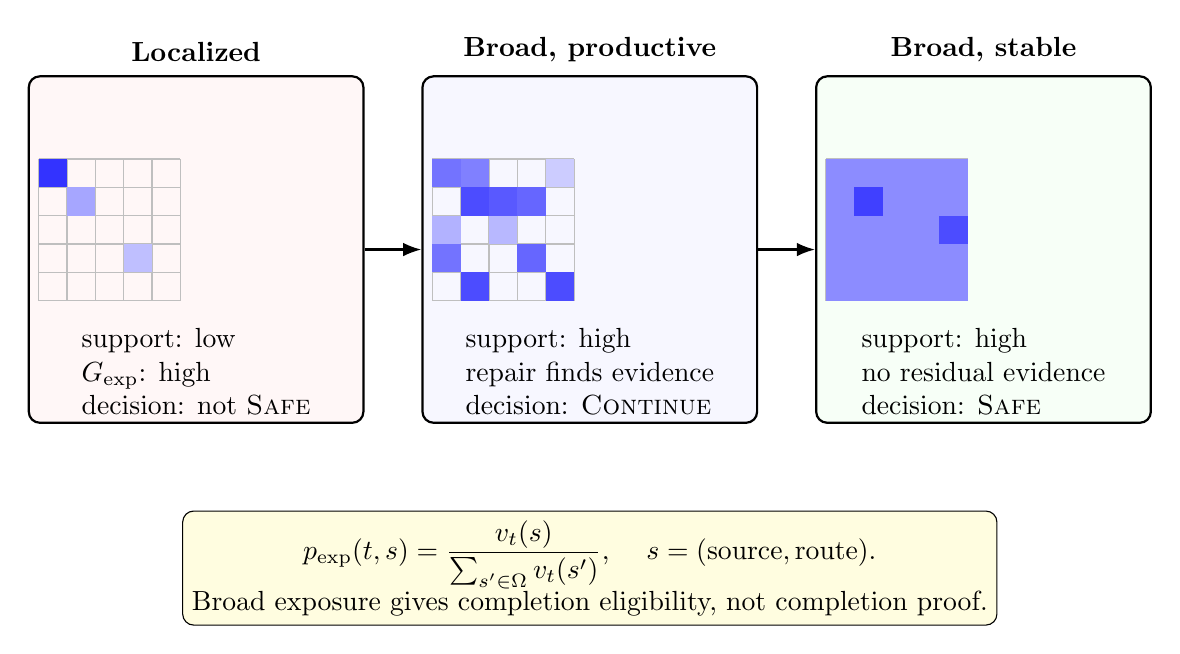
\begin{tikzpicture}[
    panel/.style={draw, rounded corners, thick, minimum width=4.25cm, minimum height=4.4cm, align=center},
    arrow/.style={-Latex, thick}
]
\newcommand{\grid}[3]{
    \begin{scope}[shift={(#1,#2)}, scale=.36]
    \foreach \i in {0,...,5} {\draw[gray!50] (0,\i) -- (5,\i); \draw[gray!50] (\i,0) -- (\i,5);}
    #3
    \end{scope}
}
\node[panel, fill=red!3] (p1) at (0,0) {};
\node[above=0.05cm of p1] {\textbf{Localized}};
\grid{-2.0}{-.65}{
    \fill[blue!80] (0,4) rectangle (1,5);
    \fill[blue!35] (1,3) rectangle (2,4);
    \fill[blue!25] (3,1) rectangle (4,2);
}
\node[align=left] at (0,-1.55) {\(\sr\): low\\\(\gexp\): high\\decision: not \safe{}};

\node[panel, fill=blue!3] (p2) at (5.0,0) {};
\node[above=0.05cm of p2] {\textbf{Broad, productive}};
\grid{3.0}{-.65}{
    \foreach \x/\y/\c in {0/4/55,1/4/50,4/4/20,1/3/70,2/3/65,3/3/60,0/2/30,2/2/28,0/1/55,3/1/60,1/0/70,4/0/70}
      {\fill[blue!\c] (\x,\y) rectangle (\x+1,\y+1);}
}
\node[align=left] at (5,-1.55) {\(\sr\): high\\repair finds evidence\\decision: \cont{}};

\node[panel, fill=green!3] (p3) at (10.0,0) {};
\node[above=0.05cm of p3] {\textbf{Broad, stable}};
\grid{8.0}{-.65}{
    \foreach \x in {0,...,4} \foreach \y in {0,...,4}
      {\fill[blue!45] (\x,\y) rectangle (\x+1,\y+1);}
    \fill[blue!75] (1,3) rectangle (2,4);
    \fill[blue!70] (4,2) rectangle (5,3);
}
\node[align=left] at (10,-1.55) {\(\sr\): high\\no residual evidence\\decision: \safe{}};

\node[draw, rounded corners, align=center, fill=yellow!12, below=1.1cm of p2,
      minimum width=10.0cm] (eq) {
      \(\displaystyle \pexp(t,s)=\frac{v_t(s)}{\sum_{s'\in\Omega}v_t(s')}\),
      \quad \(s=(\mathrm{source},\mathrm{route})\).\\
      Broad exposure gives completion eligibility, not completion proof.
};
\draw[arrow] (p1) -- (p2);
\draw[arrow] (p2) -- (p3);
\end{tikzpicture}
\caption{Source-route exposure geometry. The runtime exposure distribution over
source-route strata records where and how completion evidence was produced.
Homogeneous route reuse concentrates exposure on a small part of the coverage
simplex, so stop evidence is locally conditioned. Broader route-partitioned
exposure makes a stop claim eligible for certification, but \safe{} additionally
requires that repair or audit reveal no residual evidence.}
\label{fig:geometry}
\end{figure*}

\section{Evidence-Condition Controller}

At a proposed stop, the controller checks whether the current evidence condition
can support the stop claim. It first computes \(v_t(s)\), \(\pexp(t,s)\),
\(\sr(t)\), and \(\gexp(t)\). If the evidence condition is too localized, it
rejects \safe{} and triggers repair. A repair rule selects weak but plausible
source-route strata using only runtime-visible information. After repair, the
controller outputs \cont{} if new residual evidence appears. It outputs \safe{}
only if the evidence condition is broad and weak plausible gaps are absent. If
budget is exhausted and the certificate remains indefensible, it outputs
\abstain{}.

The controller is conservative by design. It does not infer completion merely
from confidence, agreement, or no-new evidence. It asks whether the evidence
condition is strong enough for the scope of the stop claim. In the current
implementation, support and Gini thresholds instantiate an operational
eligibility check. These thresholds are not claimed as universal laws; the
invariant is the controller structure that separates eligibility from \safe{}.

\paragraph{Residual-potential repair.}
The repair instance used in the experiments is
\[
\mathrm{priority}(s)=\mathrm{under\_exposure}(s)\cdot
\mathrm{runtime\_potential}(s).
\]
The under-exposure term gives priority to weak parts of the current completion
certificate. The runtime-potential term uses visible information such as source
text, route names, source size, route match counts, or non-oracle ledger signals.
It is not allowed to use oracle labels, oracle totals, oracle missing mass,
undiscovered true item counts, post-hoc recall, or scorer-visible target
distributions. Residual-potential is a mechanism-aligned repair instance. We do
not claim it is optimal or generally superior to all active-search alternatives.

\section{Experimental Protocol}

\paragraph{Tasks.}
We evaluate on four task families. \texttt{policy\_docset\_v1} is a generated
bounded policy document task. \texttt{code\_repo\_v1} is a generated bounded code
repository task. \texttt{requests} is an external real-repository audit over a
local snapshot of the Python \texttt{requests} package. \texttt{urllib3} is a
second external real-repository audit. The generated tasks are controlled scored
subclasses. The external tasks use real source structure but pattern-defined
oracles, so they are stronger than toy tasks and weaker than fully
human-annotated completion-audit benchmarks.

\paragraph{Conditions.}
We compare homogeneous route reuse, route-partitioned audit, and, where
available, extended or near-complete audit. Homogeneous conditions test whether
repeated local evidence can produce unsafe stop claims. Route-partitioned and
extended conditions test whether broader source-route exposure improves
completion eligibility and whether the controller can distinguish eligibility
from safety.

\paragraph{Repair challengers.}
We compare random, low-exposure, high-potential, residual-potential, and
free-search continuation challengers. These challengers are evaluated as
evidence-condition repair mechanisms, not as standalone item-finding algorithms.

\paragraph{Metrics and leakage control.}
Primary metrics are false certification, controller decision, support ratio,
exposure Gini, repair gain, cost-normalized evidence, and overlap between
high-potential and residual-potential. Recall is reported for scored subclasses,
but recall is not observed by the controller. Oracle labels are used only after
trajectories and challenger choices are fixed to score whether a stop would have
been false.

\section{Results}

\subsection{Localized Evidence Creates False Certification Risk}

Table~\ref{tab:cross} reports the main diagnostic. Across all four tasks,
homogeneous route reuse produces localized evidence conditions and would cause
false certification if accepted as \safe{}. Base support ratios range from
\(0.200\) to \(0.333\), and base exposure Gini values are high: \(0.750\) on
\texttt{code\_repo\_v1}, \(0.771\) on \texttt{policy\_docset\_v1}, \(0.889\)
on \texttt{requests}, and \(0.915\) on \texttt{urllib3}. Under the bounded
oracles, the corresponding base recalls are below the completion threshold in
all four tasks.

The controller rejects these local stops. This is the main diagnostic result:
the issue is not simply that an agent failed to find items, but that the stop
evidence was produced under a narrow source-route condition and therefore could
not support a global completion claim.

\begin{table*}[t]
\centering
\caption{Cross-task evidence-condition diagnostic. Homogeneous route reuse
produces localized exposure and would be a false certification if accepted as a
global stop in all four tasks. Broader source-route exposure improves completion
eligibility. The \texttt{urllib3} row is the boundary case: route-partitioned
exposure is broad but still incomplete, so the controller outputs \cont{} rather
than \safe{}.}
\label{tab:cross}
\resizebox{\textwidth}{!}{%
\begin{tabular}{lrrrrlrrl}
\toprule
Task & Base support & Base Gini & Base recall & False cert. & Base decision
& Broad support & Broad recall & Broad decision \\
\midrule
\texttt{policy\_docset\_v1} & 0.250 & 0.771 & 0.708 & True & \cont{} & 0.750 & 1.000 & \safe{} \\
\texttt{code\_repo\_v1}     & 0.333 & 0.750 & 0.300 & True & \cont{} & 1.000 & 0.950 & \safe{} \\
\texttt{requests}           & 0.250 & 0.889 & 0.104 & True & \cont{} & 1.000 & 1.000 & \safe{} \\
\texttt{urllib3}            & 0.200 & 0.915 & 0.193 & True & \cont{} & 0.800 & 0.835 & \cont{} \\
\bottomrule
\end{tabular}}
\end{table*}

\subsection{Broad Exposure Improves Eligibility but Does Not Guarantee Safety}

Route-partitioned evidence improves completion eligibility. In
\texttt{policy\_docset\_v1}, \texttt{code\_repo\_v1}, and \texttt{requests},
the broader condition reaches the completion threshold and the controller
outputs \safe{}. These cases show that the geometry is not merely a refusal
rule; when the evidence condition is broad and repair reveals no residual
evidence, the controller can accept the stop claim.

The \texttt{urllib3} external audit is the critical boundary case.
Route-partitioned evidence has broad support (\(0.800\)) and lower localization
than the homogeneous condition, but bounded-oracle recall is \(0.835\), below
the completion threshold. The controller outputs \cont{}, not \safe{}. An
extended audit reaches support \(1.000\), recall \(1.000\), and receives
\safe{}. This supports the intended claim: broad exposure is completion
eligibility, not a sufficient condition for safety.

\subsection{Repair Evidence Is Positive but Bounded}

Table~\ref{tab:repair} summarizes the repair boundary. Residual-potential finds
residual evidence in several tasks and is useful as a repair instance. On
\texttt{code\_repo\_v1}, it recovers more new true items than random and
high-potential in the source-route setting. On \texttt{urllib3}, it recovers
more total new evidence than high-potential. However, the method claim must
remain bounded. On \texttt{requests}, residual-potential and high-potential
select identical target sets and obtain identical gain. On \texttt{urllib3},
high-potential is similar or slightly better in cost-normalized evidence despite
lower total gain. The main conclusion does not depend on proving that the
product rule is uniquely best.

\begin{table*}[t]
\centering
\caption{Residual-potential as a bounded repair instance. Residual-potential
often finds residual evidence in weak source-route regions, but the evidence
does not establish optimality.}
\label{tab:repair}
\resizebox{\textwidth}{!}{%
\begin{tabular}{lrrrrrr}
\toprule
Task & Residual gain & High-potential gain & Random gain
& Residual/cost & High-potential/cost & Overlap \\
\midrule
\texttt{policy\_docset\_v1} & 4.000 & 0.000 & 2.025 & 0.125 & 0.000 & n/a \\
\texttt{code\_repo\_v1}     & 9.000 & 5.000 & 4.315 & 0.136 & 0.076 & n/a \\
\texttt{requests}           & 177.000 & 177.000 & 45.535 & 0.054 & 0.054 & 1.000 \\
\texttt{urllib3}            & 329.000 & 275.000 & 92.525 & 0.062 & 0.063 & 0.667 \\
\bottomrule
\end{tabular}}
\end{table*}

\begin{table}[t]
\centering
\caption{Leakage control for controller and repair decisions. Runtime decisions
use only visible evidence. Oracle labels, oracle totals, post-hoc recall, and
undiscovered true item counts are used only after trajectories and challenger
choices are fixed.}
\label{tab:leakage}
\resizebox{\columnwidth}{!}{%
\begin{tabular}{lll}
\toprule
Component & Runtime allowed & Oracle forbidden \\
\midrule
Exposure & visits, scans, actions & missing mass \\
Support/Gini & exposure counts & post-hoc recall \\
Potential & text, routes, matches & hidden true items \\
Decision & condition and repair & target distribution \\
\bottomrule
\end{tabular}}
\end{table}

\section{Limitations and Additional Validation}

The current evidence supports a diagnostic and controller in bounded
completion-audit subclasses. It does not establish a universal completion
certificate for arbitrary agent workflows. Three limitations are especially
important.

First, the external oracles are pattern-defined rather than human annotated.
They test whether the mechanism survives real repository structure, but they do
not replace a manually curated completion-audit benchmark. Second, the numeric
support and Gini thresholds are operational test points, not theory laws. Third,
source-route strata are task-designed. Different domains may require different
source and route definitions.

The most useful next experiment is not a larger version of the same table, but a
claim-verification pilot. In such a task, a workflow receives natural-language
claims over a document collection or repository and must certify whether each
claim is supported, contradicted, or unresolved. Source-route strata would pair
evidence regions with routes such as support search, contradiction search,
exception search, temporal qualification, and scope-boundary audit. This pilot
would test whether the same certificate mismatch appears when the target is not
item recall but claim support. Until it is run, it should be treated as future
validation rather than part of the current main claim.

\section{Conclusion}

This paper studies completion decisions in dynamic agent workflows under unknown
workload. The central observation is simple but consequential: local evidence
does not automatically support a global completion claim. Stop signals such as
no-new findings, agreement, or stable summaries are conditioned on where and how
the workflow searched.

Source-route evidence-condition geometry makes this conditioning explicit. The
evidence-condition controller uses that geometry to reject unsafe local stops,
repair weak plausible strata, and reserve \safe{} for cases where the evidence
condition is broad and no residual evidence appears. Across generated and
external bounded audits, homogeneous route reuse consistently creates false
certification risk, while broader source-route exposure improves completion
eligibility without being sufficient by itself. The main contribution is
therefore not a claim that a particular repair heuristic is optimal. It is a
diagnostic and control principle: completion certificates should be judged by the
evidence condition that produced them.

\bibliographystyle{plainnat}
\bibliography{references}

\clearpage
\onecolumn
\section*{Reproducibility Checklist (Draft)}

This draft includes computational experiments. The main paper states the
evaluable task families, condition types, controller metrics, and leakage
controls. A submission-ready version should add the final code archive,
environment details, seed policy, exact threshold settings, and scripts that
reproduce Tables~\ref{tab:cross}--\ref{tab:leakage}. The current experiments use
bounded generated tasks and pattern-defined external repository audits; the
paper explicitly marks human-annotated completion audits and claim-verification
pilots as future validation.

\end{document}
